\section{A Compiled Plan}\label{app:compile}
Table~\ref{tab:compile} shows one compiled plan from the test split: the predicted block values, the variant chosen for
each block, and the certificate. The compiler takes the full schemas of the highest-value tools, falls back to the
short variant (name and description only) for tools of moderate value where the full schema would not fit, and omits
blocks whose predicted value is negative.

\begin{table}[t]\centering\small
\caption{A compiled plan (tool family, Qwen3-4B-Instruct profile, 1k budget): the highest-valued optional blocks, any
other chosen blocks, and the two lowest-valued blocks, with predicted value $\hat v$ and the chosen variant.}\label{tab:compile}
\setlength{\tabcolsep}{3pt}
\fitwidth{% GENERATED by code/scripts/make_tables.py. Do not edit.
\begin{tabular}{@{}llrrl@{}}\toprule
Block & Type & Tokens & $\hat v$ & Chosen\\\midrule
\texttt{calculate\_future\_value} & tool schema & 162 & 0.447 & full\\
\texttt{calculate\_compound\_interest} & tool schema & 169 & 0.339 & full\\
\texttt{calculate\_stock\_return} & tool schema & 174 & 0.312 & full\\
\texttt{kinematics.calculate\_displacement} & tool schema & 177 & 0.106 & short\\
\texttt{biological.calc\_biomass} & tool schema & 102 & 0.103 & full\\
\texttt{finance.calculate\_quarterly\_dividend\_per\_share} & tool schema & 112 & 0.099 & full\\
\texttt{humidity\_temperature\_forecast} & tool schema & 107 & 0.080 & short\\
ex2 & example & 49 & 0.066 & full\\
\texttt{identify\_bird} & tool schema & 126 & -0.026 & --\\
ex0 & example & 52 & -0.042 & --\\
\midrule
\multicolumn{5}{@{}l}{33 optional blocks; 9 chosen; 996 of 1000 tokens; status OPTIMAL, 4.8 ms}\\
\bottomrule\end{tabular}
}
\end{table}

\section{Success Against Prompt Tokens}\label{app:frontier}
\begin{figure}[t]\centering
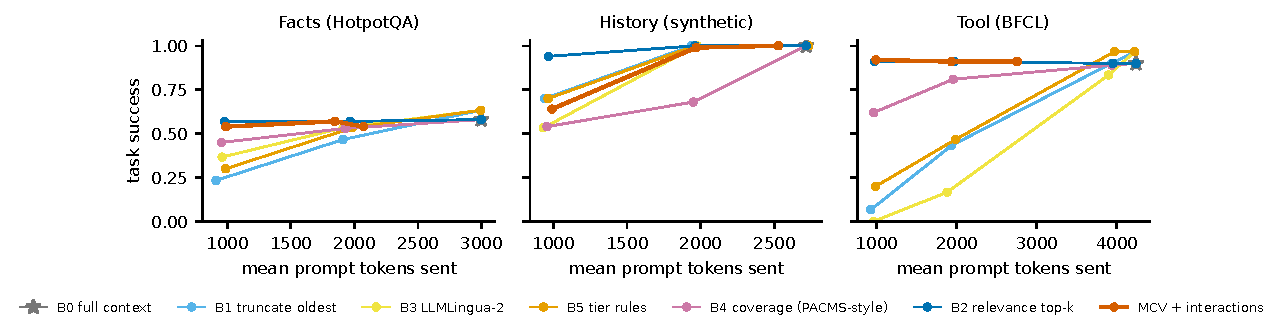
\includegraphics[width= 0.88\linewidth]{../figures/fig8_frontier.pdf}
\caption{Success against the prompt tokens actually sent (test, Qwen3-4B-Instruct; one point per budget, from 1k to 8k).
Points further left at equal height are more efficient. At its largest budget MCV sits left of full context (star) and
of B2 on tool use and history.}\label{fig:frontier}
\end{figure}

\section{Full MCV Profiles}\label{app:profiles}
\begin{table}[t]\centering\small
\caption{MCV profiles on the development split: unshrunk paired means with 95\% bootstrap CIs. Rows are type values
(success drop on removal), short-variant values (gain of the short variant over removal) and pairwise interactions.
The 8B model was profiled at type level on fewer instances, so its intervals are wider.}\label{tab:profiles}
\setlength{\tabcolsep}{3pt}
\fitwidth{% GENERATED by code/scripts/make_tables.py. Do not edit.
\begin{tabular}{@{}llcc@{}}\toprule
Family & Term & Qwen3-4B & Qwen3-8B\\\midrule
Facts & base success & 0.53 & 0.55\\
 & example & +0.05 {\scriptsize[0.00, +0.12]} & 0.00 {\scriptsize[0.00, 0.00]}\\
 & fact & +0.35 {\scriptsize[+0.17, +0.53]} & +0.35 {\scriptsize[+0.10, +0.60]}\\
 & short fact & +0.12 {\scriptsize[-0.03, +0.28]} & +0.20 {\scriptsize[0.00, +0.45]}\\
 & $I$(example, fact) & +0.10 {\scriptsize[+0.03, +0.20]} & 0.00 {\scriptsize[0.00, 0.00]}\\
\midrule
History & base success & 1.00 & 1.00\\
 & example & 0.00 {\scriptsize[0.00, 0.00]} & +0.10 {\scriptsize[0.00, +0.25]}\\
 & history turn & +0.40 {\scriptsize[+0.25, +0.55]} & +0.45 {\scriptsize[+0.25, +0.65]}\\
 & note & 0.00 {\scriptsize[0.00, 0.00]} & +0.05 {\scriptsize[0.00, +0.15]}\\
 & short history turn & -0.03 {\scriptsize[-0.12, +0.05]} & 0.00 {\scriptsize[0.00, 0.00]}\\
 & $I$(example, history turn) & 0.00 {\scriptsize[0.00, 0.00]} & +0.10 {\scriptsize[0.00, +0.25]}\\
 & $I$(example, note) & 0.00 {\scriptsize[0.00, 0.00]} & +0.10 {\scriptsize[-0.10, +0.30]}\\
 & $I$(history turn, note) & -0.60 {\scriptsize[-0.75, -0.45]} & -0.50 {\scriptsize[-0.70, -0.30]}\\
\midrule
Tool & base success & 0.85 & 0.85\\
 & example & -0.03 {\scriptsize[-0.07, 0.00]} & -0.05 {\scriptsize[-0.15, 0.00]}\\
 & tool schema & +0.85 {\scriptsize[+0.72, +0.95]} & +0.80 {\scriptsize[+0.60, +0.95]}\\
 & short tool schema & +0.30 {\scriptsize[+0.17, +0.45]} & +0.25 {\scriptsize[+0.05, +0.45]}\\
 & $I$(example, tool schema) & +0.03 {\scriptsize[-0.05, +0.10]} & 0.00 {\scriptsize[-0.15, +0.15]}\\
\bottomrule
\end{tabular}
}
\end{table}

\section{Transfer Results by Family}\label{app:transferfig}
\begin{figure}[t]\centering
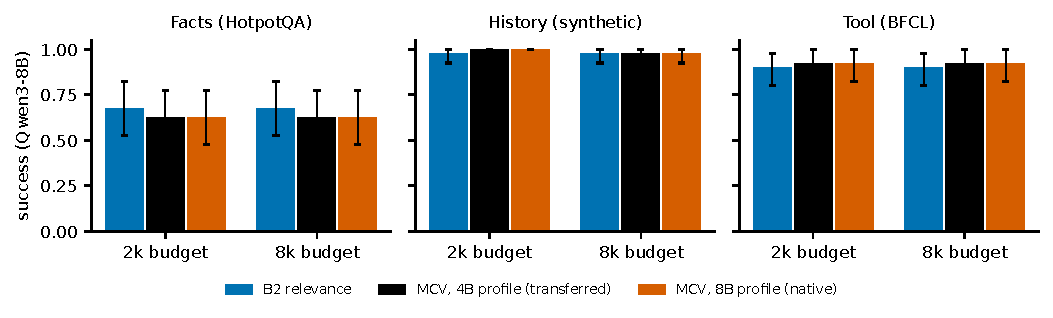
\includegraphics[width= 0.72\linewidth]{../figures/fig4_transfer.pdf}
\caption{Transfer to Qwen3-8B (test, \RNTransfer instances per family): relevance ranking, MCV with the transferred 4B
profile, and MCV with the native 8B profile, with 95\% CIs.}\label{fig:transfer}
\end{figure}

\section{Failure Analysis}\label{app:failures}
We read the transcripts of failed episodes in each family; Table~\ref{tab:excerpts} shows one representative case per
failure mode, extracted verbatim from the logs by a script. \emph{History at small budgets:} when the compiler drops the
session holding the update, the model does not guess. It reports that no conversation mentions the attribute, so these
failures are abstentions rather than hallucinations. When B2 keeps the same session, the answer is correct.
\emph{Compression of identifiers:} LLMLingua-2 deletes the underscores and reorders words in function and parameter
names. The model then emits calls whose names do not exist, which is why B3 scores far below the selection policies on
tool use at small budgets even though the call's intent is right. Selection policies never alter block text, so they
cannot fail this way. \emph{Facts with all evidence present:} in several facts losses at 8k the supporting paragraphs
were kept and only distractors were removed, yet the model's answer changed: it answered a comparison question with a
year rather than a title, or added detail that the exact-match checker rejects. Removing context changes the model's
behavior in ways a value table indexed by type cannot predict, and in these cases the change was harmful.


\begin{table}[t]\centering\small
\caption{Representative failures (test split, Qwen3-4B-Instruct), extracted verbatim from the logs. Long texts are
truncated.}\label{tab:excerpts}
% GENERATED by code/scripts/make_excerpts.py from results/raw. Do not edit.
\begin{tabular}{@{}p{0.11\textwidth}p{0.45\textwidth}p{0.4\textwidth}@{}}\toprule
Case & Goal and context & Replies (verbatim)\\\midrule
History, 1k & Question: What is the user's current car? Session holding the update: ``User: "By the way, I drive a white Tesla Model 3 now."''. Kept by B2: yes; by MCV: no. & \texttt{\footnotesize MCV: ANSWER: None of the provided conversations mention the user's current car.}\newline \texttt{\footnotesize B2: ANSWER: white Tesla Model 3}\\
Tool, 1k & Request: Calculate the future value of my investment of \$1000 with an annual interest rate of 5\% over 2 years. & \texttt{\footnotesize MCV: \{"name": "calculate\_future\_value", "arguments": \{"initial\_investment": 1000, "interest\_rate": 0.05, "duration": 2\}\}}\newline \texttt{\footnotesize B3: \{"name": "calculate future value", "arguments": \{"investment initial": "1000", "yearly interest": "5", "compounded": "1", "holding period": "2"\}\}}\\
Facts, 8k & Question: Which film was released first out of The Hunchback of Notre Dame and Miracle of the White Stallions? & \texttt{\footnotesize MCV: ANSWER: 1963}\newline \texttt{\footnotesize B0: ANSWER: Miracle of the White Stallions}\\
\bottomrule\end{tabular}

\end{table}

\section{How Much Profiling Is Needed?}\label{app:samplesize}
Profiling cost scales with the number of development instances, so we asked, again as an exploratory analysis of the
existing logs, how quickly the type-level profile stabilizes. We re-estimated the 4B profiles from random subsets of
the \RNProfFour profiled instances (\RSsDraws draws per size) and compared them with the full-sample profile
(Fig.~\ref{fig:samplesize}). With five instances per family the mean absolute error of the type values was \RSsMaeFive and
the most valuable type was identified in all three families in \RSsTopFive of draws. With ten instances these were
\RSsMaeTen and \RSsTopTen, and with twenty \RSsMaeTwenty and \RSsTopTwenty. Because subsets are drawn from the same
\RNProfFour instances, agreement at larger sizes is partly mechanical. The practical reading is that the type-level ranking
needs on the order of ten to twenty instances per family, while the block-level model would need far more informative
supervision than single-block deletions provide.

\begin{figure}[t]\centering
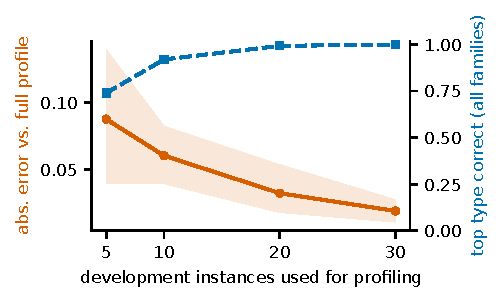
\includegraphics[width= 0.72\linewidth]{../figures/fig7_sample_size.pdf}
\caption{Profile stability versus development instances (exploratory; subsamples of the 4B profiling logs). Band: the
range of the middle four fifths of draws.}\label{fig:samplesize}
\end{figure}

\section{Development History}\label{app:devhistory}
The block-value model went through three versions on development data only. The first used lexical features (dev AUBC
\RDevAubcOne); the second added embedding similarity (\RDevAubcTwo); the third, which apportioned type value across
blocks, scored \RDevAubcThree and was rejected by the rule fixed before it ran. The second version was frozen and
pre-registered before any test run. All three pilots, and a crashed pilot run, are in the released logs.
